\documentclass[11pt,a4paper]{article}
\usepackage[utf8]{inputenc}
\usepackage[T2A,T1]{fontenc}
\usepackage[english]{babel}
\usepackage{geometry}
\geometry{margin=2.2cm}
\usepackage{longtable,booktabs,array}
\usepackage{hyperref}
\hypersetup{colorlinks=true,linkcolor=blue,urlcolor=blue}
\usepackage{listings}
\lstset{
  basicstyle=\ttfamily\small,
  breaklines=true,
  frame=single,
  backgroundcolor=\color[gray]{0.96},
  columns=fullflexible,
  keepspaces=true
}
\usepackage{xcolor}
\usepackage{enumitem}
\setlist{nosep}

\title{\textbf{MBS-raw: Physical Optics for Ice Crystals}\\[4pt]\large Manual}
\author{}
\date{2026-03-22}

\begin{document}
\maketitle
\tableofcontents
\newpage

%======================================================================
\section{Overview}

MBS-raw computes light scattering by non-spherical particles using the Physical Optics (PO) method.
It traces geometric optics rays through the particle (reflections, refractions),
then applies Kirchhoff diffraction to each output beam to obtain the far-field Mueller matrix.

\textbf{Optimized version}: $\sim$70$\times$ faster than original. AVX-512/AVX2 SIMD, OpenMP parallel,
Sobol quasi-random orientations. Builds for Intel, AMD Zen\,2 (EPYC 7H12), and AMD Zen\,4 (Ryzen 7000 / EPYC Genoa).

%======================================================================
\section{Quick Start}

\begin{lstlisting}
# Simple run: hex column, Sobol orientations, auto theta grid
mbs_po --po --sobol 1024 --auto_tgrid \
    -p 1 10 10 -w 0.532 --ri 1.31 0 -n 12 \
    --grid 0 180 48 180 --close

# Fully adaptive (auto everything)
mbs_po --po --adaptive 0.01 --auto_tgrid \
    -p 1 10 10 -w 0.532 --ri 1.31 0 -n 12 \
    --grid 0 180 48 180 --close
\end{lstlisting}

%======================================================================
\section{CLI Reference}

All flags are grouped by function. Required flags have no default; optional flags are marked with their defaults.

%----------------------------------------------------------------------
\subsection{Particle Definition}

\subsubsection{\texttt{-p TYPE HEIGHT DIAMETER [EXTRA]}}

\begin{tabular}{lll}
\toprule
Type & Shape & Parameters \\
\midrule
1  & Hexagonal column   & H = height, D = diameter \\
2  & Bullet             & H, D (cap angle 62\textdegree, auto) \\
3  & Bullet rosette     & H, D, [cap height] \\
4  & Droxtal            & arg3 = sup parameter \\
10 & Concave hexagonal  & H, D, concavity depth \\
12 & Hexagonal aggregate & H, D, number of elements \\
\bottomrule
\end{tabular}

\textbf{Symmetry}: auto-detected. Hex column: $\beta_\text{sym}=\pi/2$, $\gamma_\text{sym}=\pi/3$ $\to$ 12$\times$ reduction.

\subsubsection{\texttt{--pf FILENAME}}
Load particle geometry from file. \texttt{-p} argument provides the filename.

\subsubsection{\texttt{--rs SIZE}}
Resize particle loaded with \texttt{--pf} to maximal dimension SIZE ($\mu$m).

\subsubsection{\texttt{--forced\_convex} / \texttt{--forced\_nonconvex}}
Force convex or non-convex tracing algorithm.

%----------------------------------------------------------------------
\subsection{Physical Parameters}

\subsubsection{\texttt{-w WAVELENGTH\_UM}}
Wavelength in micrometers. Examples: \texttt{-w 0.532} (green), \texttt{-w 1.064} (NIR).

\subsubsection{\texttt{--ri N\_REAL N\_IMAG}}
Complex refractive index $m = n_\text{re} + i\,n_\text{im}$.\\
\textbf{Important}: Without \texttt{--abs}, imaginary part is forced to zero.

\subsubsection{\texttt{--abs}}
Enable absorption. Requires \texttt{-w}. Uses \texttt{DiffractInclineAbs}.

\subsubsection{\texttt{-n MAX\_REFLECTIONS}}

\begin{tabular}{lll}
\toprule
Value & Use case & Notes \\
\midrule
5--6  & Forward scattering, $C_\text{sca}$ & $<1\%$ error \\
12    & General purpose & $<5\%$ backscatter error \\
20    & Backscattering & $<3\%$ error \\
25    & Reference calculations & \\
\bottomrule
\end{tabular}

%----------------------------------------------------------------------
\subsection{Method}

\begin{itemize}
\item \texttt{--po} --- Physical Optics (Kirchhoff diffraction). \textbf{Required for PO.}
\item \texttt{--go} --- Geometrical Optics (no diffraction).
\item \texttt{--incoh} --- Incoherent summation ($|J|^2$ per beam, then sum).
\item \texttt{--karczewski} --- Karczewski polarization matrix (experimental, same $M_{11}$).
\item \texttt{--jones} --- Output Jones matrices to file.
\item \texttt{--all} --- Compute all trajectory groups.
\end{itemize}

%----------------------------------------------------------------------
\subsection{Orientations}

\subsubsection{\texttt{--sobol N} (recommended)}
$N$ Sobol quasi-random orientations (power of 2). Auto-uses particle symmetry.\\
Convergence: $O((\log N)^2/N)$, much faster than Monte Carlo $O(1/\sqrt{N})$.

\begin{tabular}{lll}
\toprule
$x$ & $C_\text{sca}$ ($<2\%$) & $M_{11}(180\degree)$ ($<5\%$) \\
\midrule
10--50   & 128  & 512 \\
50--200  & 256  & 1024 \\
200--1000 & 512 & 4096 \\
$>1000$  & 1024 & 8192+ \\
\bottomrule
\end{tabular}

\subsubsection{\texttt{--adaptive EPS}}
Auto-determine orientations. Starts at 256, doubles until $C_\text{sca}$ converges to relative accuracy EPS.

\subsubsection{\texttt{--sym B G}}
Override particle symmetry: $\beta \in [0, \pi/B]$, $\gamma \in [0, 2\pi/G]$.\\
Example: \texttt{--sym 6 2} $\to$ $\beta\in[0,30\degree]$, $\gamma\in[0,180\degree]$ (12$\times$ reduction).

\subsubsection{Other orientation modes}
\begin{itemize}
\item \texttt{--random N\_BETA N\_GAMMA} --- Uniform grid.
\item \texttt{--montecarlo N} --- Random orientations.
\item \texttt{--fixed BETA GAMMA} --- Single orientation (degrees).
\item \texttt{--orientfile FILE} --- Read $(\beta,\gamma)$ pairs (radians) from file.
\item \texttt{-b MIN MAX}, \texttt{-g MIN MAX} --- Override ranges (degrees).
\end{itemize}

%----------------------------------------------------------------------
\subsection{Scattering Grid}

\subsubsection{\texttt{--grid T1 T2 N\_PHI N\_THETA}}
Uniform grid. \textbf{Use $N_\phi \geq 48$}; $N_\phi=6$ causes 50--200\% error.

\subsubsection{\texttt{--auto\_tgrid} (recommended)}
Auto non-uniform $\theta$ grid with 5 adaptive zones:

\begin{tabular}{llll}
\toprule
Zone & Range & Step & Purpose \\
\midrule
Fine & $0$ to $10\times$peak & peak$/20$ & Forward peak \\
Transition & to $20\degree$ & geometric $\times 1.3$ & Smooth bridging \\
Medium & to $120\degree$ & $0.5\degree$ ($x{<}100$) or $1\degree$ & Side scattering \\
Side/back & to $175\degree$ & $1\degree$ & Backscattering \\
Near-backscatter & to $180\degree$ & $0.25\degree$ & LDR \\
\bottomrule
\end{tabular}

\begin{figure}[h]\centering
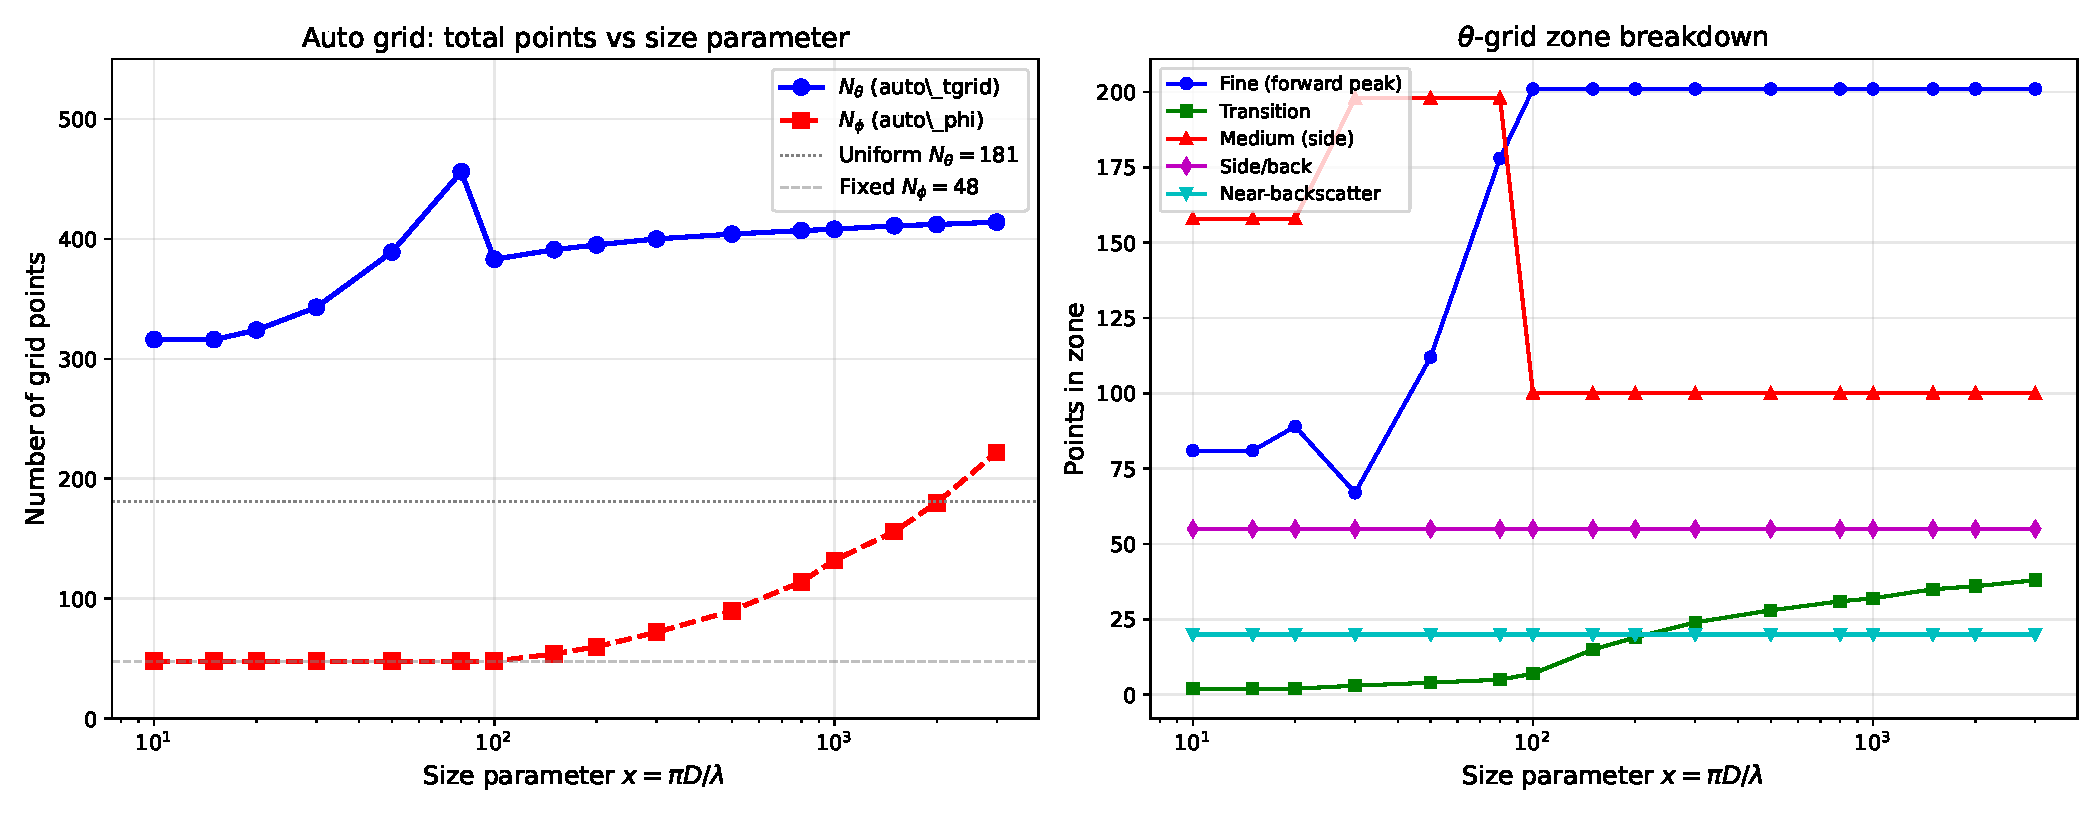
\includegraphics[width=\textwidth]{fig_auto_grid_points.pdf}
\caption{Left: total $N_\theta$ and $N_\phi$ vs size parameter $x$.
Right: zone breakdown of $\theta$-grid points.}
\end{figure}

\begin{figure}[h]\centering
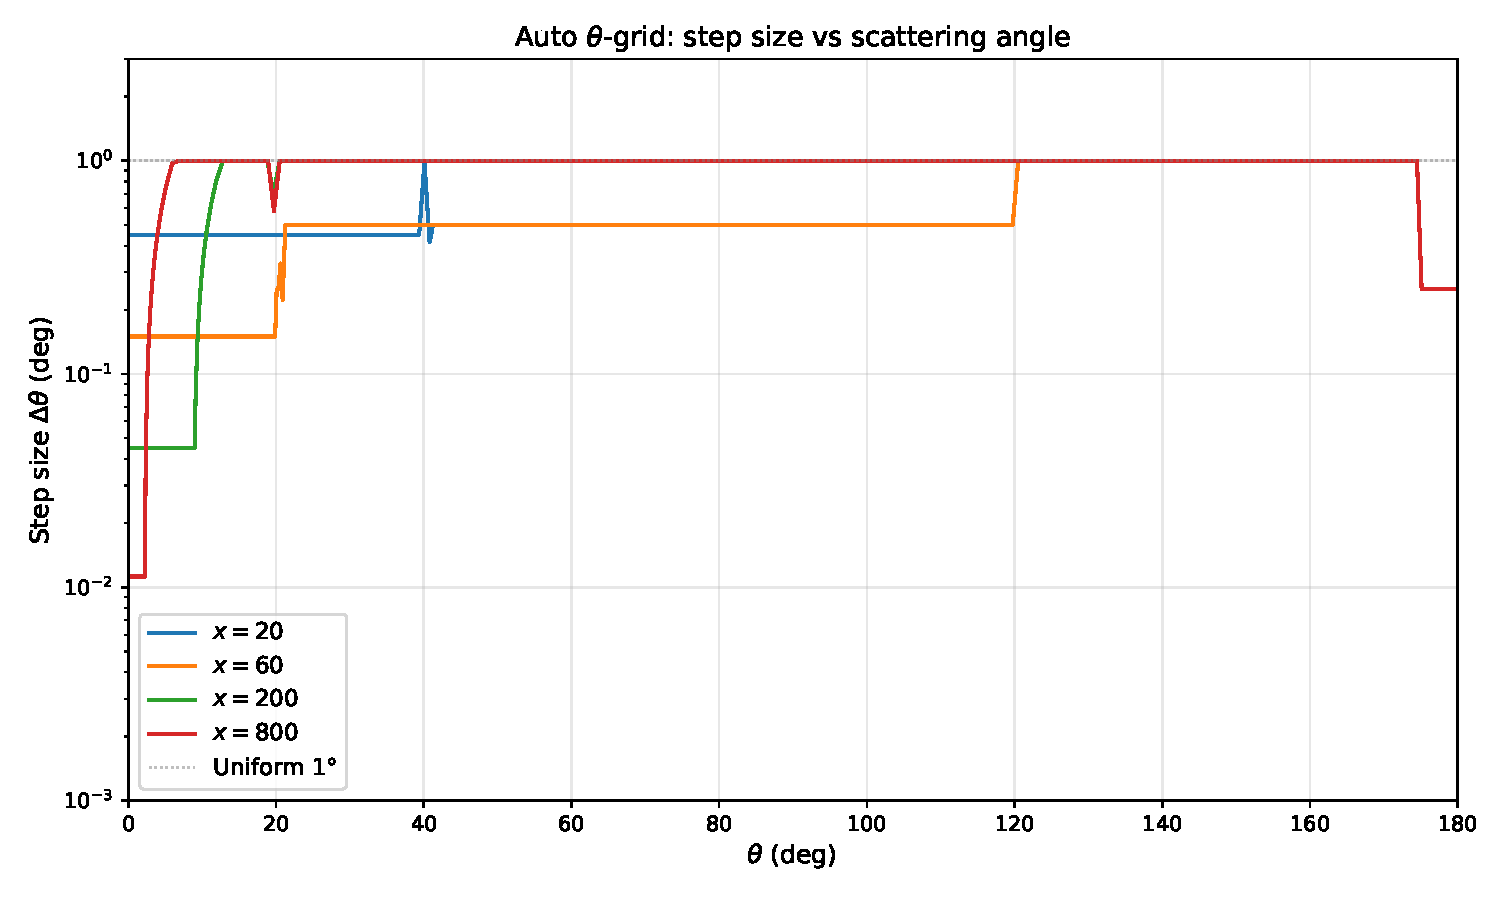
\includegraphics[width=0.85\textwidth]{fig_auto_grid_steps.pdf}
\caption{Step size $\Delta\theta$ vs scattering angle for different $x$.
Small $x$ has coarser steps (broad peak); large $x$ needs fine steps near $\theta{=}0$.}
\end{figure}

\subsubsection{\texttt{--auto\_phi}}
Auto-select $N_\phi$ based on $x$: $N_\phi = \max(48,\; 6\lceil\sqrt{x}/1.5\rceil)$.

\begin{figure}[h]\centering
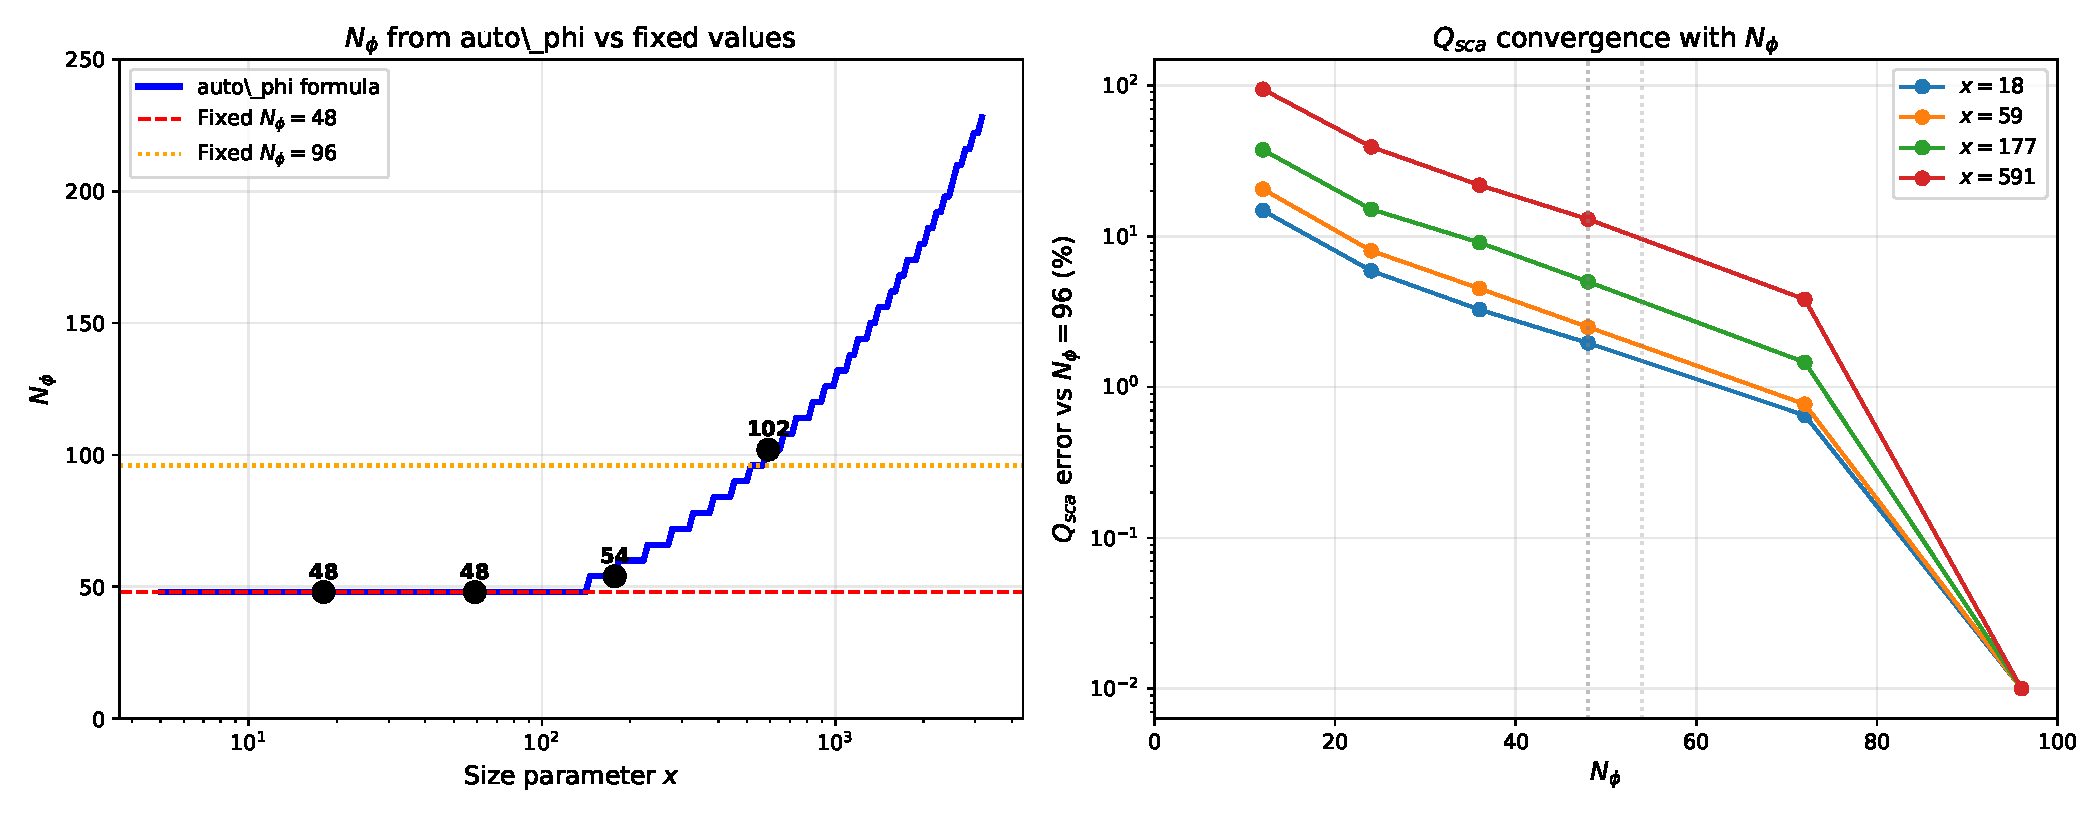
\includegraphics[width=\textwidth]{fig_auto_phi.pdf}
\caption{Left: $N_\phi$ from auto\_phi (blue) vs fixed values.
Right: $Q_\text{sca}$ error vs $N_\phi$ for different sizes—larger $x$ needs more $\phi$ bins.}
\end{figure}

\textbf{Recommended}: use both \texttt{--auto\_tgrid --auto\_phi} together.

\subsubsection{\texttt{--tgrid FILENAME}}
Custom $\theta$ grid from file (degrees, one per line).

%----------------------------------------------------------------------
\subsection{Multi-Size (\texttt{--sizefile})}

\begin{lstlisting}
--sizefile sizes.txt   # one x = pi*D/lambda per line
\end{lstlisting}

Traces beams once, caches geometry, recomputes diffraction for each size.
Output: \texttt{M\_x10.dat}, \texttt{M\_x20.dat}, etc.

%----------------------------------------------------------------------
\subsection{Performance Options}

\begin{itemize}
\item \texttt{--beam\_cutoff EPS} --- Skip negligible beams.
\item \texttt{--shadow\_off} --- Disable shadow beam (debug).
\item \texttt{-r RATIO} --- Small beam restriction ratio (default 100).
\end{itemize}

%----------------------------------------------------------------------
\subsection{Output}

\begin{itemize}
\item \texttt{-o DIRNAME} --- Output folder (default \texttt{M}).
\item \texttt{--close} --- Exit after calculation (\textbf{required for scripts}).
\item \texttt{--log SECONDS} --- Progress output interval.
\item \texttt{--tr FILE} --- Trajectory groups from file.
\item \texttt{--gr} --- Per-group output.
\end{itemize}

%======================================================================
\section{Output Files}

\subsection{M.dat}

Tab-separated columns:
\begin{lstlisting}
theta  2pi*dcos  M11  M12  M13  M14  M21  M22  M23  M24  ...  M44
\end{lstlisting}

$C_\text{sca} = \sum M_{11} \times (2\pi\,d\cos\theta)$.

%======================================================================
\section{Build}

\subsection{Intel / AVX-512}
\begin{lstlisting}
bash build.sh            # -> bin/mbs_po
\end{lstlisting}
\texttt{-O3 -march=native -mavx512f -mavx512dq -fopenmp}. Requires GCC $\geq$ 9.

\subsection{AMD EPYC 7H12 (Zen 2, SP3)}
\begin{lstlisting}
bash build_epyc.sh       # -> bin/mbs_po_epyc
bash build_epyc_clang.sh # -> bin/mbs_po_epyc_clang
\end{lstlisting}
\texttt{-march=znver2}. No AVX-512; \texttt{fast\_sincos\_8x} falls back to $2\times$\texttt{fast\_sincos\_4x}.

\textbf{NUMA}: \texttt{OMP\_PROC\_BIND=close OMP\_PLACES=cores OMP\_NUM\_THREADS=64}

\subsection{AMD Zen 4 (Ryzen 7000, EPYC Genoa)}
\begin{lstlisting}
bash build_zen4.sh       # -> bin/mbs_po_zen4
\end{lstlisting}
\texttt{-march=znver4 -mavx512f -mavx512dq -mavx512vl}.

\subsection{Generic AVX2}
Remove \texttt{-mavx512*} from \texttt{build.sh}. Code auto-detects via \texttt{\#ifdef \_\_AVX512F\_\_}.

%======================================================================
\section{Performance}

\subsection{Single-thread benchmarks}

Hex $D{=}H{=}10\,\mu$m, 128 Sobol, $48\,\phi \times 181\,\theta$, $n{=}6$:

\begin{tabular}{lrl}
\toprule
Version & Phase 2 & vs Original \\
\midrule
Original (before optimizations) & $\sim$320\,s & 1$\times$ \\
Optimized + batched sincos      & 4.6\,s & \textbf{$\sim$70$\times$} \\
EPYC build (AVX2 only)          & 4.7\,s & $\sim$68$\times$ \\
\bottomrule
\end{tabular}

\subsection{Key optimizations}
\begin{enumerate}
\item \textbf{PrecomputeEdgeData}: slopes, intercepts computed once per beam (not per direction).
\item \textbf{Theta-coefficients}: $A(\theta) = \sin\theta\cdot a_s + \cos\theta\cdot a_c + a_0$ (2 FMA).
\item \textbf{Batched sincos}: all vertex phases for all $\theta$ pre-computed before the $\theta$-loop. AVX-512 \texttt{fast\_sincos\_8x} or AVX2 $2\times$\texttt{fast\_sincos\_4x}.
\item \textbf{Polynomial sincos}: Cody--Waite range reduction + Chebyshev polynomial ($\sim$14 decimal digits).
\item \textbf{Inline hot loop}: no heap allocation, stack-only \texttt{complex} arithmetic.
\item \textbf{OpenMP}: thread-local Mueller accumulators, \texttt{schedule(dynamic,1)}.
\item \textbf{Sobol + symmetry}: native C++ Sobol generator with particle symmetry reduction.
\end{enumerate}

\subsection{OpenMP scaling}

\begin{tabular}{lrl}
\toprule
Threads & Phase 2 & Speedup \\
\midrule
1          & 4.6\,s & 1.0$\times$ \\
4          & 1.7\,s & 2.7$\times$ \\
12 (SMT)   & $\sim$0.9\,s & $\sim$5$\times$ \\
64 (EPYC)  & $\sim$0.2\,s* & $\sim$23$\times$* \\
\bottomrule
\end{tabular}

*Estimated; use $\geq$512 orientations for 64 cores.

%======================================================================
\section{Bugfixes}

\subsection{Forward-direction Fresnel sign (2026-03-22)}

\textbf{Bug}: sign error in the forward-direction special case ($A{\approx}0, B{\approx}0$) of the Kirchhoff integral.
The edge-sum converges to $-F_\text{inv}\cdot\text{area}$ but the shortcut used $+F_\text{inv}\cdot\text{area}$.

\textbf{Symptom}: $M_{11}(0\degree)$ anomalously small in coherent mode for small particles.
Example (hex $D{=}H{=}3\,\mu$m): $M_{11}(0)/M_{11}(0.1\degree) = 0.019$ (should be $\approx 1.03$).

\textbf{Fix}: negate the forward-direction formula in 6 locations:
\begin{itemize}
\item \texttt{HandlerPO.cpp}: lines 970, 1333, 1889
\item \texttt{Handler.cpp}: lines 255, 473, 642
\end{itemize}

Incoherent mode unaffected ($|J|^2$ is sign-independent).
$Q_\text{sca}$ changed by $\sim$0.06\%.
See \texttt{BUGFIX\_forward\_direction\_sign.md} for full details.

%======================================================================
\section{Known Limitations}

\begin{enumerate}
\item \textbf{$Q_\text{sca} > 2$ at large $x$}: PO does not enforce the optical theorem.
\item \textbf{$M_{33}, M_{34}, M_{44}$}: RotateJones vs Karczewski give different off-diagonal elements (same $M_{11}$).
\item \textbf{Small particles ($x < 20$)}: PO not valid. Use ADDA or T-matrix.
\item \textbf{Backscattering convergence}: $M_{11}(180\degree)$ needs 10--100$\times$ more orientations.
\item \textbf{LTO}: \texttt{-flto} causes $\sim$20\% regression. Do not use.
\end{enumerate}

%======================================================================
\section{File Listing}

\begin{tabular}{ll}
\toprule
File & Description \\
\midrule
\texttt{build.sh}             & Intel/AVX-512 build \\
\texttt{build\_epyc.sh}       & AMD EPYC 7H12 (Zen 2) build \\
\texttt{build\_epyc\_clang.sh} & EPYC + Clang/AOCC build \\
\texttt{build\_zen4.sh}        & AMD Zen 4 (Ryzen 7000/Genoa) build \\
\texttt{Makefile}              & Legacy Makefile (Intel) \\
\texttt{Makefile.epyc}         & Makefile for EPYC \\
\texttt{tests/run\_tests.sh}   & Regression test suite \\
\texttt{MANUAL.md}             & This manual (Markdown source) \\
\texttt{BUGFIX\_forward\_direction\_sign.md} & Bugfix documentation \\
\bottomrule
\end{tabular}

\end{document}
